\xchapter{Evaluation}{}
\label{cap:evaluation}

In this chapter we evaluate JVMTIPROF by using it to instrument Elasticsearch. We adapt a profile-guided frequency scaling solution~\cite{hurryupccgrid} to use JVMTIPROF instead of JVMTI. We then measure the overhead and identify whether JVMTIPROF can produce the same gains as the baseline despite its abstractions.

\section{Experimental Setup}

We conducted our experiments on a baremetal server instance, provided by the Chameleon Cloud service. The server consists of an Intel Xeon Gold 6126 (Skylake architecture), with 196GB of DRAM and a 220GB SSD disk.  We run Ubuntu 20.04 (Linux kernel 5.4) and Elasticsearch version 6.5.4. For the search index database, we used the Wikipedia dump version \code{enwiki-latest-pages-articles} downloaded in September, 2022.

The CPU has 24 physical cores equally divided between two sockets. Intel’s Hyperthreading technology was turned off, so we only consider the physical core count. To isolate the network effects in the shared experimental platform, we configured socket 0 to run the server-side applications (Elasticsearch) and socket 1 to execute the load generator (FABAN).

The energy measurement was done through Intel’s Running Average Power Limit (RAPL) interface. We measured the energy consumption counter at the beginning of the experiment and at the end; the difference between those two values is considered the energy consumed for that particular experiment.

The client (FABAN~\cite{faban}) is responsible to generate query requests with randomized keywords, ranging between 1 to 18 keywords, under a Zipfian distribution, as explained in~\cite{hurryupccgrid}.

The load generation process consisted of 20 minutes runs of continuous search queries. The FABAN workload generator was used to create 4 clients with each client issuing, on average, one request per second. The goal was to analyze the behavior of each solution considering a single request at a time. An additional configuration of three times the requests-per-seconds is used to explore loads similar to that of production environments.

We performed six runs for each combination of load and solution and reported the standard deviation.

% TODO p99

\section{Baseline}

The Linux Ondemand power governor and Hurryup~\cite{hurryupccgrid} are used as baselines for our experiments. Hurryup is a profile-guided frequency scaling solution for Elasticsearch that outperforms Ondemand on energy consumption while attaining acceptable levels of tail latency constraints.

Hurryup works by instrumenting Elasticsearch's hot functions to produce enter and exit events. These events are used by a run-time scheme to adapt the individual processor core frequencies. In our experiments, we observed Hurryup saving up to 25\% in energy compared to Linux's Ondemand governor, as seen in Figure~\ref{fig:ondem_vs_hup}.

\begin{figure}[hb]
\centering
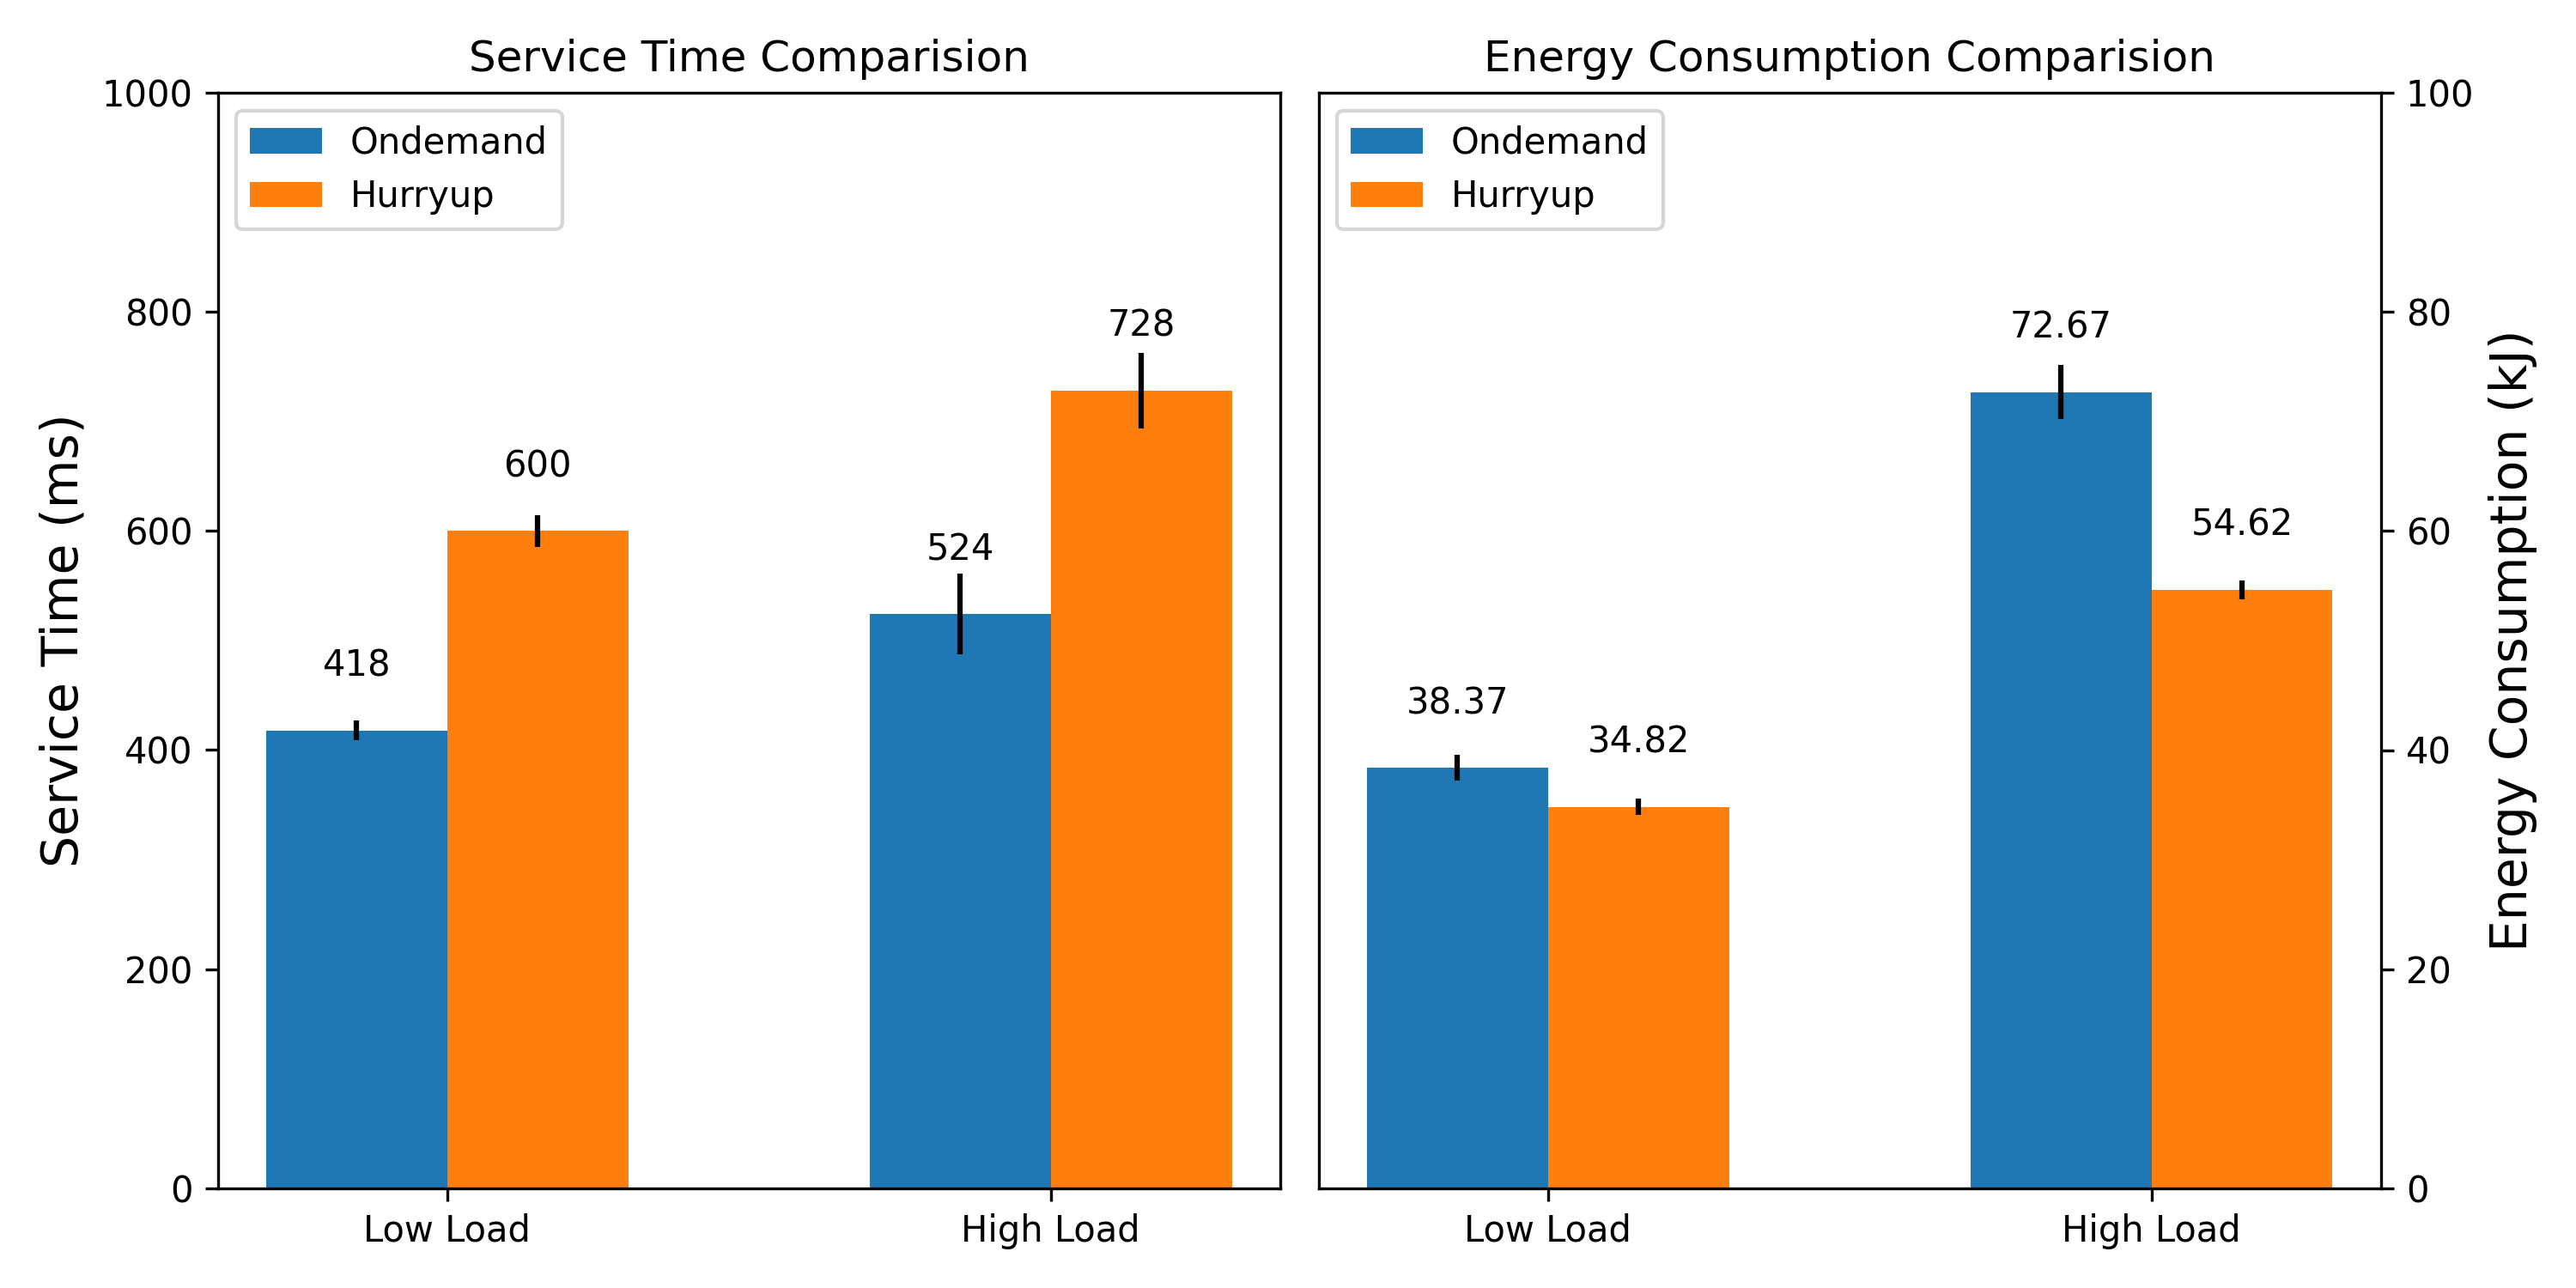
\includegraphics[width=1.0\textwidth]{src/figure/ondem_vs_hup.png}
\caption{An experiment comparing Linux's Ondemand governor against Hurryup's frequency scaling scheme. The left plot presents Elasticsearch's service time and the right plot the energy consumption of the CPU while executing search requests. Results are shown for both a low and high server load.}
\label{fig:ondem_vs_hup}
\end{figure}

\section{Results}

% 1X LOAD HUP vs NEWHUP is statistically significant
% 1X LOAD ENERGY HUP vs NEWHUP is not SS
% 3X LOAD HUP vs NEWHUP is not SS
% 3X LOAD ENERGY HUP vs NEWHUP is SS
% 1X LOAD ENERGY ONDEMAND vs (HUP, NEWHUP) = 9% gain
% 3X LOAD ENERGY ONDEMAND vs NEWHUP = 22.75% gain

We modify Hurryup to use JVMTIPROF's instrumentation methods and re-execute the experiments as reported in Figure~\ref{fig:ondem_vs_hup_vs_newhup}. We notice that JVMTIPROF can be similar or slightly worse than JVMTI in the context of Hurryup, but can still achieve energy gains compared to Ondemand while meeting the service time deadline.

\begin{figure}[ht]
\centering
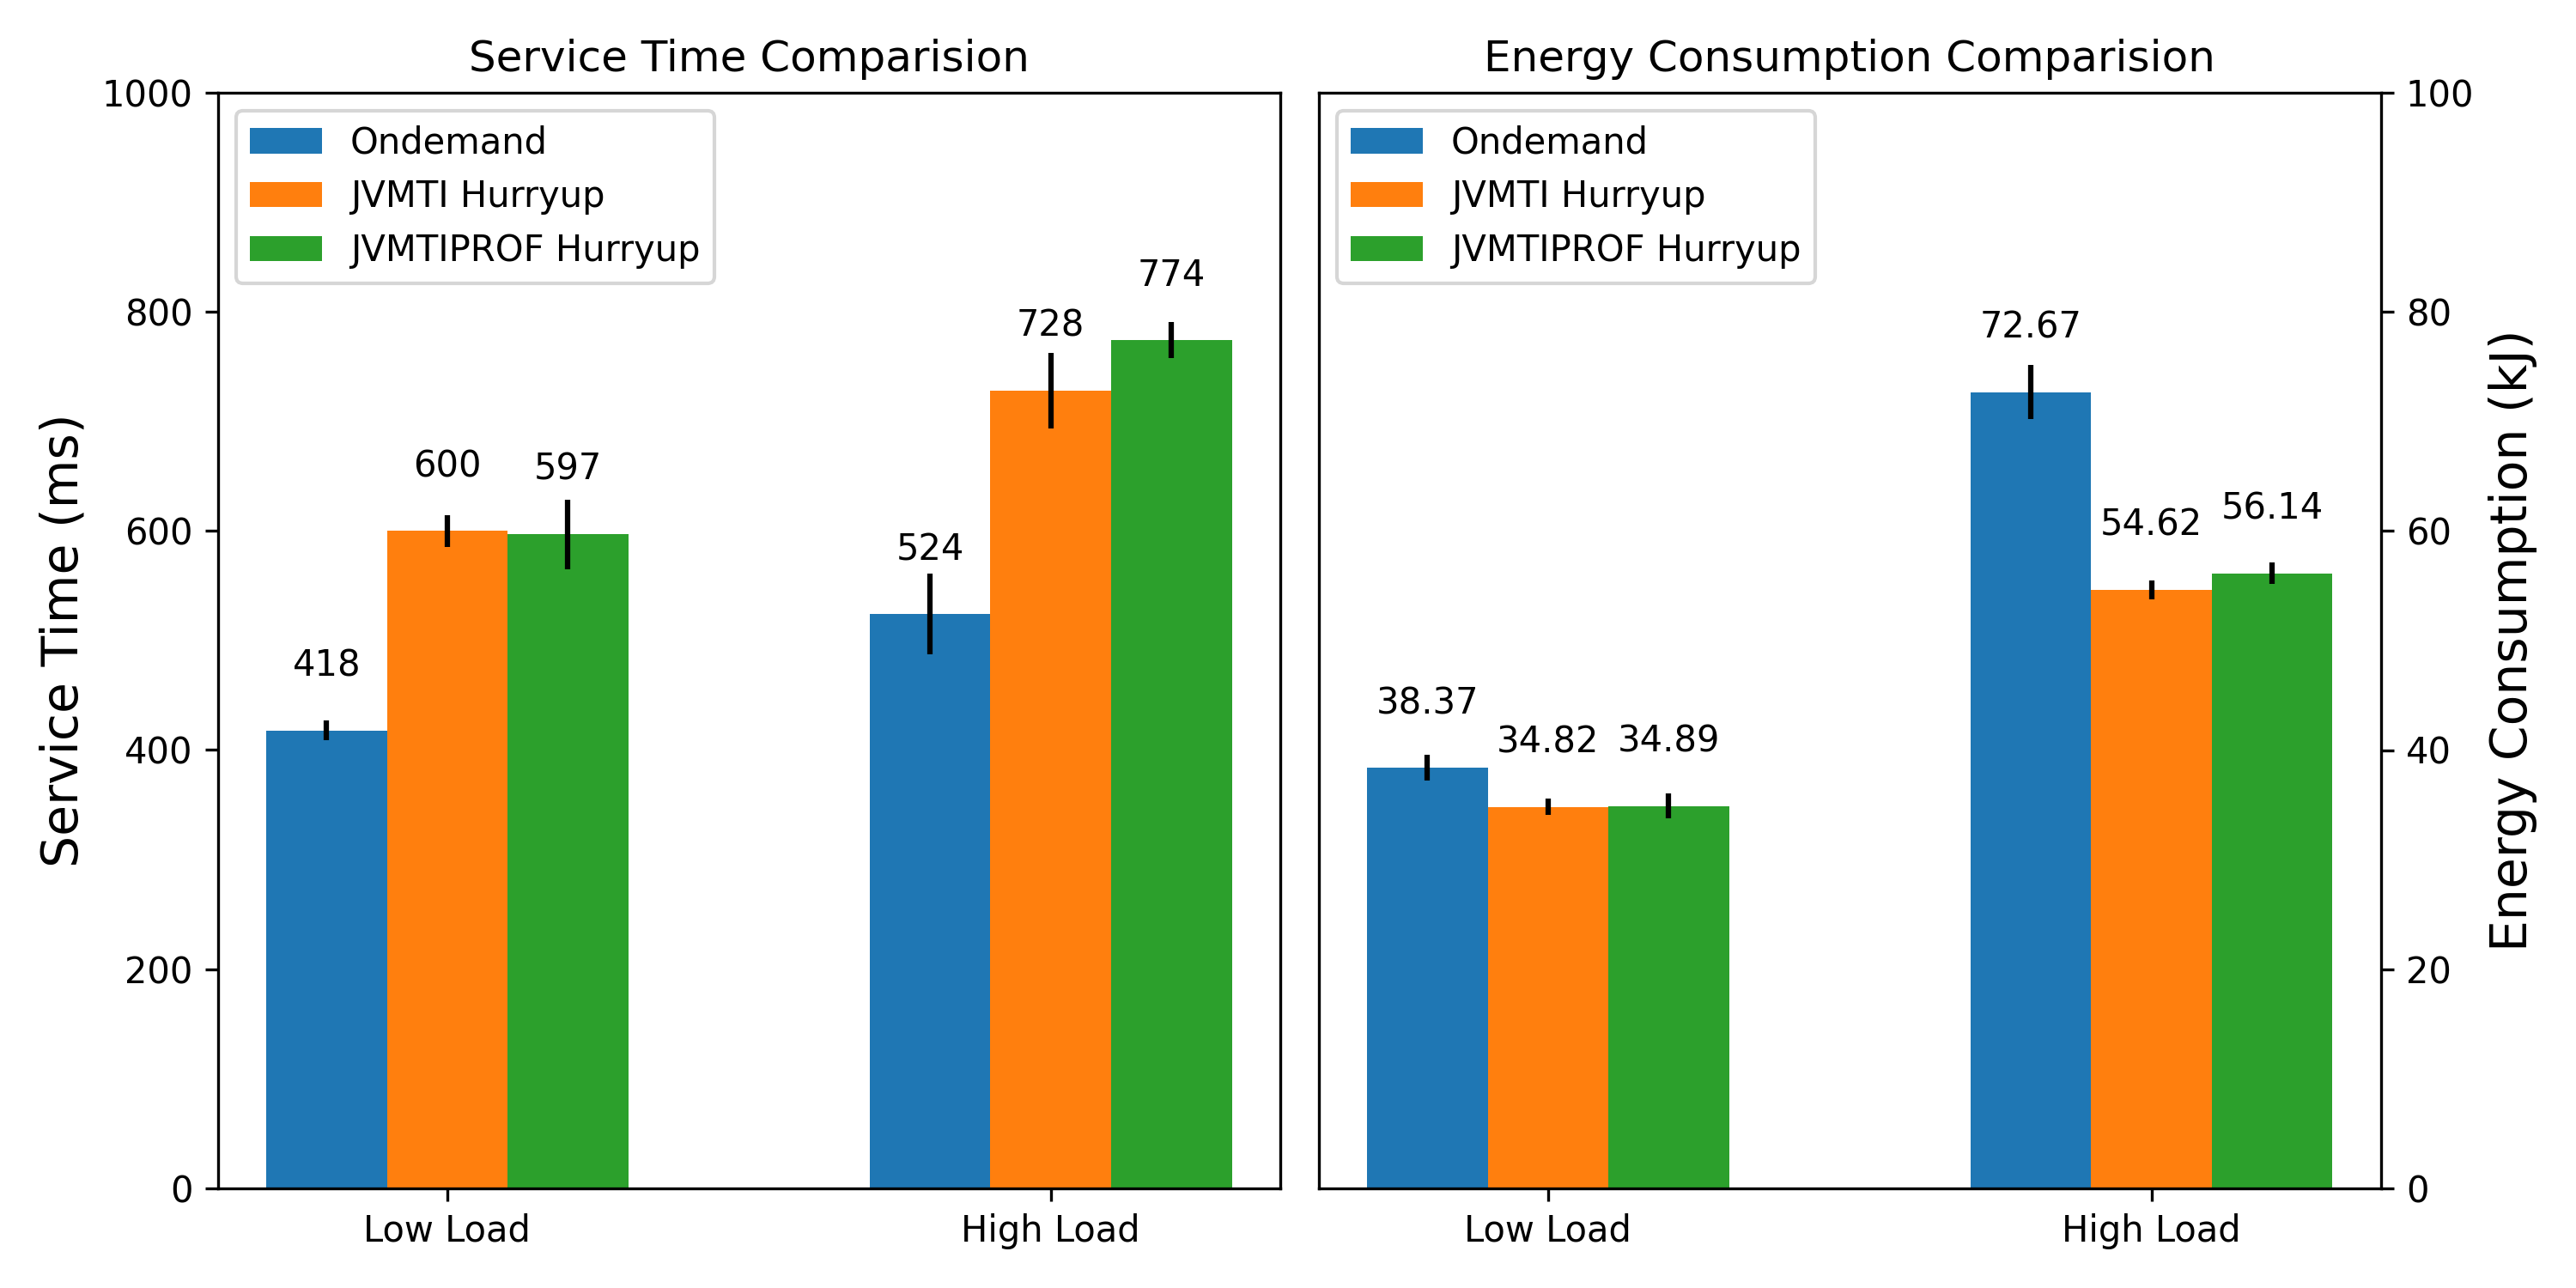
\includegraphics[width=1.0\textwidth]{src/figure/ondem_vs_hup_vs_newhup.png}
\caption{An experiment comparing Hurryup's performance when implemented with JVMTIPROF versus the baseline. The left plot presents Elasticsearch's service time and the right plot the energy consumption of the CPU while executing search requests. Results are shown for both a low and high server load.}
\label{fig:ondem_vs_hup_vs_newhup}
\end{figure}

At a lower load, the JVMTI and JVMTIPROF implementations do not present a statistically significant difference in both service time and energy consumption. When tripling the load, the JVMTIPROF version can be 6\% worse in service time and 2.78\% worse in energy consumption.

We also compare the overhead of instrumenting Elasticsearch's hot functions, excluding Hurryup specific logic. Results are presented in Figure~\ref{fig:overhead}. There is no statistically significant difference between instrumenting or not instrumenting said functions, with either JVMTI or JVMTIPROF.

\begin{figure}[ht]
\centering
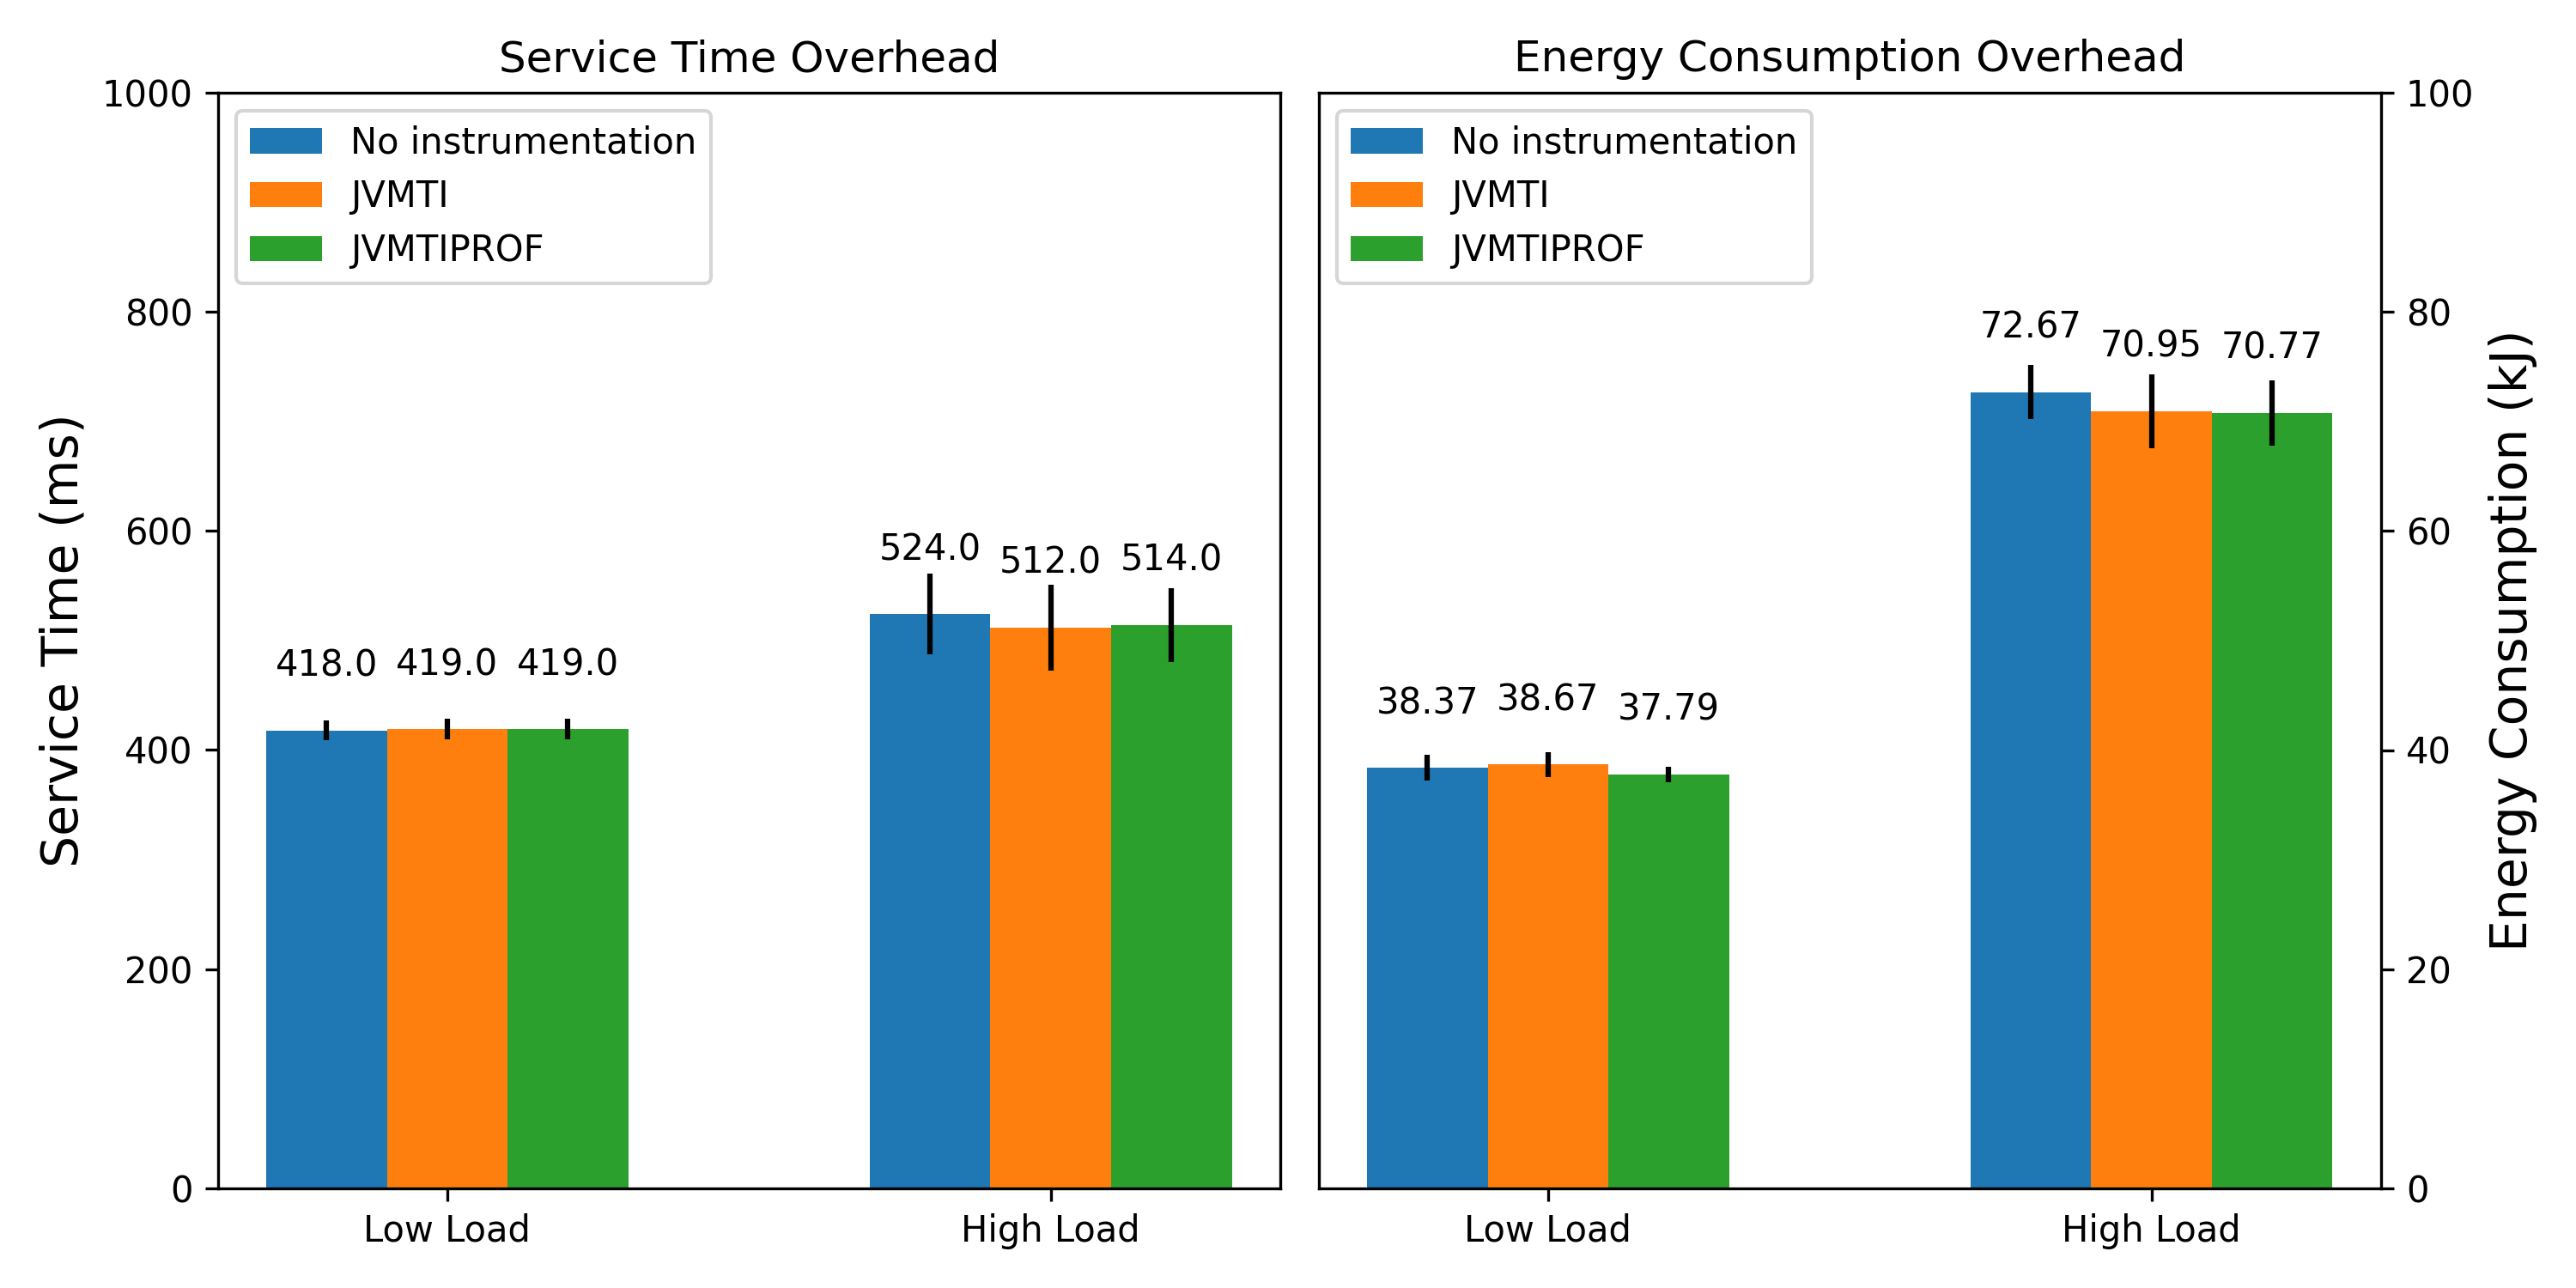
\includegraphics[width=1.0\textwidth]{src/figure/overhead.png}
\caption{An experiment comparing the performance of Elasticsearch when their hot functions are kept as-is or hooked with JVMTI and JVMTIPROF. The left plot presents Elasticsearch's service time and the right plot the energy consumption of the CPU while executing search requests. Results are shown for both a low and high server load.}
\label{fig:overhead}
\end{figure}

These results also show that the context in which the instrumentation is used may cause performance differences. When instrumenting to run Hurryup logic at a higher load, JVMTIPROF performed worse than JVMTI, but at lower loads or with no additional logic present, no difference is available.
